% Options for packages loaded elsewhere
\PassOptionsToPackage{unicode}{hyperref}
\PassOptionsToPackage{hyphens}{url}
\PassOptionsToPackage{dvipsnames,svgnames,x11names}{xcolor}
%
\documentclass[
  letterpaper,
  DIV=11,
  numbers=noendperiod,
  oneside]{scrreprt}

\usepackage{amsmath,amssymb}
\usepackage{iftex}
\ifPDFTeX
  \usepackage[T1]{fontenc}
  \usepackage[utf8]{inputenc}
  \usepackage{textcomp} % provide euro and other symbols
\else % if luatex or xetex
  \usepackage{unicode-math}
  \defaultfontfeatures{Scale=MatchLowercase}
  \defaultfontfeatures[\rmfamily]{Ligatures=TeX,Scale=1}
\fi
\usepackage{lmodern}
\ifPDFTeX\else  
    % xetex/luatex font selection
\fi
% Use upquote if available, for straight quotes in verbatim environments
\IfFileExists{upquote.sty}{\usepackage{upquote}}{}
\IfFileExists{microtype.sty}{% use microtype if available
  \usepackage[]{microtype}
  \UseMicrotypeSet[protrusion]{basicmath} % disable protrusion for tt fonts
}{}
\makeatletter
\@ifundefined{KOMAClassName}{% if non-KOMA class
  \IfFileExists{parskip.sty}{%
    \usepackage{parskip}
  }{% else
    \setlength{\parindent}{0pt}
    \setlength{\parskip}{6pt plus 2pt minus 1pt}}
}{% if KOMA class
  \KOMAoptions{parskip=half}}
\makeatother
\usepackage{xcolor}
\usepackage[left=1in,marginparwidth=2.0666666666667in,textwidth=4.1333333333333in,marginparsep=0.3in]{geometry}
\ifLuaTeX
  \usepackage{luacolor}
  \usepackage[soul]{lua-ul}
\else
  \usepackage{soul}
  
\fi
\setlength{\emergencystretch}{3em} % prevent overfull lines
\setcounter{secnumdepth}{5}
% Make \paragraph and \subparagraph free-standing
\makeatletter
\ifx\paragraph\undefined\else
  \let\oldparagraph\paragraph
  \renewcommand{\paragraph}{
    \@ifstar
      \xxxParagraphStar
      \xxxParagraphNoStar
  }
  \newcommand{\xxxParagraphStar}[1]{\oldparagraph*{#1}\mbox{}}
  \newcommand{\xxxParagraphNoStar}[1]{\oldparagraph{#1}\mbox{}}
\fi
\ifx\subparagraph\undefined\else
  \let\oldsubparagraph\subparagraph
  \renewcommand{\subparagraph}{
    \@ifstar
      \xxxSubParagraphStar
      \xxxSubParagraphNoStar
  }
  \newcommand{\xxxSubParagraphStar}[1]{\oldsubparagraph*{#1}\mbox{}}
  \newcommand{\xxxSubParagraphNoStar}[1]{\oldsubparagraph{#1}\mbox{}}
\fi
\makeatother


\providecommand{\tightlist}{%
  \setlength{\itemsep}{0pt}\setlength{\parskip}{0pt}}\usepackage{longtable,booktabs,array}
\usepackage{calc} % for calculating minipage widths
% Correct order of tables after \paragraph or \subparagraph
\usepackage{etoolbox}
\makeatletter
\patchcmd\longtable{\par}{\if@noskipsec\mbox{}\fi\par}{}{}
\makeatother
% Allow footnotes in longtable head/foot
\IfFileExists{footnotehyper.sty}{\usepackage{footnotehyper}}{\usepackage{footnote}}
\makesavenoteenv{longtable}
\usepackage{graphicx}
\makeatletter
\newsavebox\pandoc@box
\newcommand*\pandocbounded[1]{% scales image to fit in text height/width
  \sbox\pandoc@box{#1}%
  \Gscale@div\@tempa{\textheight}{\dimexpr\ht\pandoc@box+\dp\pandoc@box\relax}%
  \Gscale@div\@tempb{\linewidth}{\wd\pandoc@box}%
  \ifdim\@tempb\p@<\@tempa\p@\let\@tempa\@tempb\fi% select the smaller of both
  \ifdim\@tempa\p@<\p@\scalebox{\@tempa}{\usebox\pandoc@box}%
  \else\usebox{\pandoc@box}%
  \fi%
}
% Set default figure placement to htbp
\def\fps@figure{htbp}
\makeatother

\KOMAoption{captions}{tableheading}
\makeatletter
\@ifpackageloaded{tcolorbox}{}{\usepackage[skins,breakable]{tcolorbox}}
\@ifpackageloaded{fontawesome5}{}{\usepackage{fontawesome5}}
\definecolor{quarto-callout-color}{HTML}{909090}
\definecolor{quarto-callout-note-color}{HTML}{0758E5}
\definecolor{quarto-callout-important-color}{HTML}{CC1914}
\definecolor{quarto-callout-warning-color}{HTML}{EB9113}
\definecolor{quarto-callout-tip-color}{HTML}{00A047}
\definecolor{quarto-callout-caution-color}{HTML}{FC5300}
\definecolor{quarto-callout-color-frame}{HTML}{acacac}
\definecolor{quarto-callout-note-color-frame}{HTML}{4582ec}
\definecolor{quarto-callout-important-color-frame}{HTML}{d9534f}
\definecolor{quarto-callout-warning-color-frame}{HTML}{f0ad4e}
\definecolor{quarto-callout-tip-color-frame}{HTML}{02b875}
\definecolor{quarto-callout-caution-color-frame}{HTML}{fd7e14}
\makeatother
\makeatletter
\@ifpackageloaded{bookmark}{}{\usepackage{bookmark}}
\makeatother
\makeatletter
\@ifpackageloaded{caption}{}{\usepackage{caption}}
\AtBeginDocument{%
\ifdefined\contentsname
  \renewcommand*\contentsname{Tabla de contenidos}
\else
  \newcommand\contentsname{Tabla de contenidos}
\fi
\ifdefined\listfigurename
  \renewcommand*\listfigurename{Listado de Figuras}
\else
  \newcommand\listfigurename{Listado de Figuras}
\fi
\ifdefined\listtablename
  \renewcommand*\listtablename{Listado de Tablas}
\else
  \newcommand\listtablename{Listado de Tablas}
\fi
\ifdefined\figurename
  \renewcommand*\figurename{Figura}
\else
  \newcommand\figurename{Figura}
\fi
\ifdefined\tablename
  \renewcommand*\tablename{Tabla}
\else
  \newcommand\tablename{Tabla}
\fi
}
\@ifpackageloaded{float}{}{\usepackage{float}}
\floatstyle{ruled}
\@ifundefined{c@chapter}{\newfloat{codelisting}{h}{lop}}{\newfloat{codelisting}{h}{lop}[chapter]}
\floatname{codelisting}{Listado}
\newcommand*\listoflistings{\listof{codelisting}{Listado de Listados}}
\makeatother
\makeatletter
\makeatother
\makeatletter
\@ifpackageloaded{caption}{}{\usepackage{caption}}
\@ifpackageloaded{subcaption}{}{\usepackage{subcaption}}
\makeatother
\makeatletter
\@ifpackageloaded{sidenotes}{}{\usepackage{sidenotes}}
\@ifpackageloaded{marginnote}{}{\usepackage{marginnote}}
\makeatother

\ifLuaTeX
\usepackage[bidi=basic]{babel}
\else
\usepackage[bidi=default]{babel}
\fi
\babelprovide[main,import]{spanish}
% get rid of language-specific shorthands (see #6817):
\let\LanguageShortHands\languageshorthands
\def\languageshorthands#1{}
\usepackage{bookmark}

\IfFileExists{xurl.sty}{\usepackage{xurl}}{} % add URL line breaks if available
\urlstyle{same} % disable monospaced font for URLs
\hypersetup{
  pdftitle={Introducción a la Economía con Aplicaciones para República Dominicana},
  pdfauthor={Frank Fuentes, Julio Andujar y Oscar Pascual},
  pdflang={es},
  colorlinks=true,
  linkcolor={blue},
  filecolor={Maroon},
  citecolor={Blue},
  urlcolor={Blue},
  pdfcreator={LaTeX via pandoc}}


\title{Introducción a la Economía con Aplicaciones para República
Dominicana}
\author{Frank Fuentes, Julio Andujar y Oscar Pascual}
\date{2026-03-06}

\begin{document}
\maketitle

\renewcommand*\contentsname{Tabla de contenidos}
{
\hypersetup{linkcolor=}
\setcounter{tocdepth}{2}
\tableofcontents
}

\bookmarksetup{startatroot}

\chapter*{Prefacio}\label{prefacio}
\addcontentsline{toc}{chapter}{Prefacio}

\markboth{Prefacio}{Prefacio}

La economía está presente en cada decisión cotidiana: cuando una familia
organiza su presupuesto mensual, cuando una empresa decide invertir,
cuando el gobierno diseña una política pública o cuando un país negocia
su inserción en el comercio internacional. Sin embargo, a pesar de su
presencia constante en la vida social, la economía suele percibirse como
un campo técnico, distante y complejo.

Este libro nace con un objetivo sencillo: presentar los principios
fundamentales de la economía de forma clara, rigurosa y accesible,
utilizando como referencia constante la realidad de la República
Dominicana.

Durante las últimas décadas, la economía dominicana ha experimentado
transformaciones profundas. El país ha transitado desde una economía
fuertemente dependiente de la agricultura hacia una estructura más
diversificada basada en servicios, turismo, zonas francas, comercio y
construcción. Al mismo tiempo, enfrenta retos estructurales importantes:
desigualdad, informalidad laboral, sostenibilidad fiscal, vulnerabilidad
climática y la necesidad de elevar la productividad.

Comprender estos procesos requiere más que la simple observación de
datos o indicadores. Requiere un marco conceptual que permita
interpretar cómo funcionan los mercados, cómo toman decisiones los
individuos y las empresas, y cómo interactúan las políticas públicas con
el comportamiento económico.

Ese marco conceptual es lo que proporciona la teoría económica.

Este libro introduce al lector a los principios fundamentales de la
economía ---escasez, incentivos, mercados, competencia, crecimiento,
inflación, comercio internacional y política económica--- utilizando
ejemplos, instituciones y experiencias propias del contexto dominicano
siempre que sea posible. La intención no es únicamente explicar
conceptos abstractos, sino mostrar cómo esas ideas ayudan a entender
fenómenos reales: desde el funcionamiento del mercado laboral hasta la
política monetaria del Banco Central, desde la dinámica del turismo
hasta los efectos del comercio internacional.

La obra está organizada en tres grandes secciones.

La primera sección presenta los fundamentos del pensamiento económico:
qué estudia la economía, cómo se construyen los modelos y cuáles son los
principios básicos que permiten analizar decisiones bajo condiciones de
escasez.

La segunda sección se centra en la microeconomía, es decir, en el
comportamiento de los agentes individuales: consumidores, empresas y
mercados. Se examinan los mecanismos de oferta y demanda, la formación
de precios, las decisiones de consumo y producción, las diferentes
estructuras de mercado y las situaciones en las que los mercados pueden
fallar.

La tercera sección aborda la macroeconomía, el estudio de la economía en
su conjunto. Allí se analizan temas como el producto interno bruto, la
inflación, el desempleo, el sistema financiero, el crecimiento
económico, los ciclos económicos, el comercio internacional y el papel
de las políticas fiscal y monetaria.

A lo largo del texto se busca mantener un equilibrio entre intuición
económica, herramientas analíticas y aplicaciones empíricas. El objetivo
no es únicamente que el lector memorice conceptos, sino que desarrolle
una forma de pensar: el razonamiento económico.

Pensar como economista implica formular preguntas, identificar
incentivos, reconocer restricciones y analizar cómo las decisiones
individuales interactúan dentro de sistemas más amplios. Esta forma de
análisis resulta útil no solo para quienes estudian economía, sino
también para estudiantes de administración, finanzas, políticas
públicas, derecho y ciencias sociales en general.

Finalmente, este libro parte de una convicción fundamental: comprender
la economía es una herramienta esencial para participar de manera
informada en el debate público. Las decisiones económicas ---sobre
impuestos, gasto público, regulación, comercio o política monetaria---
afectan directamente el bienestar de la sociedad. Una ciudadanía con
mayor comprensión económica puede contribuir a discusiones públicas más
rigurosas y a decisiones colectivas mejor fundamentadas.

Si este libro logra que el lector observe la realidad económica
dominicana con mayor curiosidad, espíritu crítico y capacidad analítica,
entonces habrá cumplido su propósito.

\part{Fundamentos}

\chapter{Qué es la economía}\label{quuxe9-es-la-economuxeda}

\section{Objetivo del cápitulo}\label{objetivo-del-cuxe1pitulo}

\begin{itemize}
\item
  Mostrar la relevancia de la economía en la vida cotidiana, destacando
  cómo las decisiones personales, empresariales y gubernamentales en la
  República Dominicana están condicionadas por la escasez y los precios.
\item
  Definir qué estudia la economía como ciencia social, explicando su
  objeto de estudio: la asignación de recursos escasos para satisfacer
  necesidades ilimitadas.
\item
  Introducir los conceptos fundamentales del análisis económico, como
  escasez, elección, costo de oportunidad, eficiencia, incentivos y
  pensamiento marginal.
\item
  Explicar los principios básicos del comportamiento económico racional,
  incluyendo la optimización, la toma de decisiones marginales y los
  errores comunes como la falacia del costo hundido.
\item
  Presentar las principales áreas y enfoques de la economía,
  distinguiendo entre microeconomía y macroeconomía, así como entre el
  enfoque positivo y el normativo.
\end{itemize}

\section{Introducción}\label{introducciuxf3n}

\textbf{``¡Es la Economía, estúpido!''}

Esta fue la famosa frase que fue clave para la inesperada victoria para
el expresidente de los Estados Unidos Bill Clinton en las elecciones de
1992. Todas las predicciones apuntaban a una reelección de George H. W.
Bush padre, cuya popularidad rondaba el 90\% gracias a sus éxitos en
materia de política exterior con el fin de la Guerra Fría y la guerra
del Golfo. El enfoque estratégico de la campaña de Clinton se centró en
cuestiones más relacionadas con la vida cotidiana de la ciudadanía y sus
necesidades más inmediatas.

De la misma manera, la economía sigue teniendo una alta vinculación con
nuestra cotidianidad a nivel personal o empresarial, ya que nos ayuda a
comprender cómo las personas, las empresas y el Estado toman decisiones
en un contexto de recursos limitados. Lejos de ser una disciplina
abstracta o exclusivamente académica, la economía está presente en
acciones tan simples como decidir qué comprar en el supermercado,
aceptar un empleo, ahorrar parte del salario o evaluar si es conveniente
endeudarse.

Cuando los dominicanos observan que los precios de los alimentos, el
transporte o la electricidad suben, están experimentando los efectos de
la inflación, una variable económica que impacta directamente el poder
adquisitivo de sus salarios. Asimismo, la economía es clave para la toma
de decisiones personales y familiares. En un país donde muchas familias
dependen de remesas, créditos de consumo o préstamos hipotecarios, el
conocimiento económico ayuda a comprender el costo real del
endeudamiento, la importancia del ahorro y los riesgos asociados a las
tasas de interés. La economía también es esencial para comprender cuando
el gobierno anuncia inversiones en infraestructura o una reforma fiscal,
se están tomando decisiones económicas que afectan a toda la sociedad.

En conclusión, el estudio de la economía no solo es importante para
especialistas, sino para cualquier ciudadano que aspire a tomar
decisiones informadas y a participar de manera consciente en la vida
económica y social del país.

\section{¿Qué estudia la economía?}\label{quuxe9-estudia-la-economuxeda}

La economía como área de estudio parte de una simple observación: los
recursos disponibles (financieros, naturales, humanos, etc.) son
limitados, pero los deseos de las personas (necesidades, aspiraciones,
etc.) no lo son. Por ende, es necesario hacer el uso más eficiente
posible de los recursos disponibles para satisfacer la mayor cantidad de
necesidades de las personas. Como señalan Samuelson y Nordhaus (XXXX),
la economía surge precisamente porque la sociedad no puede producir todo
lo que las personas necesitan y desean al mismo tiempo. En este contexto
la economía puede definirse como:

\begin{quote}
\textbf{La ciencia social que estudia la manera en que los individuos,
las empresas y los países deciden utilizar sus recursos escasos para
satisfacer sus necesidades.}
\end{quote}

\subsection{Escasez: el punto de
partida}\label{escasez-el-punto-de-partida}

La escasez es uno de los conceptos centrales de la economía y constituye
el punto de partida para comprender cómo funcionan las sociedades. En
términos simples, la escasez se refiere a la situación en la que los
recursos disponibles ---como el tiempo, el dinero, la tierra, el trabajo
o el capital--- son limitados, mientras que las necesidades y deseos
humanos son prácticamente ilimitados.

La escasez no es pobreza, ya que incluso los países, empresas y personas
son impactados por ella. La escasez significa que solo existe una
cantidad finita y limitada de recursos disponibles. Debido a esta
realidad, no es posible producir todo lo que las personas quieren en las
cantidades que desean, lo que obliga a tomar decisiones y a establecer
prioridades.

La escasez también explica por qué los precios existen y cumplen un rol
tan importante. En una economía, los precios actúan como señales que
reflejan la escasez relativa de los bienes y servicios. Cuando un
producto es escaso en relación con la demanda, su precio tiende a subir,
incentivando a los productores a ofrecer más y a los consumidores a
usarlo con mayor cuidado. De esta forma, la escasez contribuye a la
asignación eficiente de los recursos. Comprender la realidad de la
escasezpermite analizar estas decisiones de manera más realista y ya que
todas las soluciones implican costos.

Por ejemplo, el gobierno dominicano enfrenta demandas crecientes de
gasto en educación, salud, seguridad e infraestructura, pero dispone de
ingresos limitados provenientes de impuestos y endeudamiento. Esta
restricción obliga a priorizar: invertir más en transporte público puede
significar menos recursos para otros programas sociales.

Asimismo, aunque la economía dominicana ha crecido en las últimas
décadas, los empleos bien remunerados y con protección social siguen
siendo limitados en relación con la oferta de trabajadores. Esto explica
la persistencia de la informalidad laboral y las diferencias salariales
entre sectores como turismo, zonas francas y comercio informal.

En conclusión, la escasez es una realidad estructural que condiciona las
decisiones de individuos, empresas y del Estado en la República
Dominicana. Entender su papel permite analizar mejor los problemas
económicos del país y tomar decisiones más informadas tanto a nivel
personal como colectivo.

\subsection{Necesidades: el objetivo
final}\label{necesidades-el-objetivo-final}

Las necesidades pueden ser definidas son aquellos bienes y servicios
indispensables para la supervivencia y el bienestar básico de las
personas, como la alimentación, la vivienda, la salud y la educación.
Los deseos, en cambio, representan aspiraciones o preferencias que van
más allá de lo esencial y que están influenciadas por la cultura, el
ingreso, la publicidad y el entorno social.

Adam Smith, considerado el padre de la Economía, ya observaba en su
libro ``La Riqueza de las Naciones'' que lo que una sociedad considera
``necesario'' cambia con el tiempo y el contexto social. En economías
modernas, bienes que antes eran considerados lujos ---como el acceso a
internet o un celular--- se han convertido en necesidades prácticas para
participar en el mercado laboral y en la vida social. Esto demuestra que
las necesidades y deseos son dinámicos y tienden a expandirse con el
crecimiento del ingreso y el desarrollo económico.

En la República Dominicana, muchas familias utilizan prácticamente todo
su ingreso mensual para cubrir necesidades básicas como alimentos,
transporte y electricidad. Sin embargo, a medida que el ingreso aumenta,
surgen deseos adicionales, como adquirir un vehículo, mudarse a un lugar
más espacioso o irse de vacaciones fuera del país.

\subsection{Elección: el proceso de tomar
decisiones}\label{elecciuxf3n-el-proceso-de-tomar-decisiones}

En economía, la combinación de recursos escasos y deseos ilimitados es
la base del problema fundamental de la elección. Dado que las personas,
las empresas y los gobiernos no disponen de recursos suficientes para
satisfacer todos sus deseos al mismo tiempo, se ven obligados a
elegirentre alternativas. Estas elecciones no son aleatorias, sino que
responden a un proceso racional orientado a obtener el mayor beneficio
posible dadas las restricciones existentes. A este proceso se le conoce
en economía como optimización.

La optimización consiste en seleccionar la mejor opción posible de entre
un conjunto de alternativas, considerando una restricción
presupuestaria, de tiempo o de recursos productivos. Por ejemplo, un
consumidor quisiera consumir una amplia variedad de bienes, pero su
ingreso es limitado. Frente a esta restricción, debe decidir cómo
asignar su presupuesto para maximizar su satisfacción.

Este mismo razonamiento se aplica a las empresas. Toda compañía se crea
con el objetivo de generar beneficios. Sin embargo, enfrentan las
limitaciones de los recursos necesarios para producir. Por ende, deben
elegir comprar la combinación óptima de materia prima que minimiza
costos o maximiza producción. Así, la escasez obliga a las empresas a
optimizar sus decisiones productivas y de inversión.

En el ámbito del sector público, la elección también está también
condicionada por la escasez. Los gobiernos enfrentan grandes demandas
sociales (mejor educación, salud, seguridad e infraestructura) pero
cuentan con recursos fiscales limitados. La optimización se traduce
entonces en asignar el presupuesto público de manera que maximice el
bienestar social, sujeto a restricciones fiscales y políticas.

En conclusión, la coexistencia de recursos escasos y deseos ilimitados
hace inevitable la elección económica. La optimización proporciona el
marco analítico para entender cómo los agentes toman decisiones
racionales, comparan alternativas y asignan recursos de la forma más
eficiente posible dentro de sus limitaciones.

\subsection{La economía como ciencia: Definiciones clásicas y
modernas}\label{la-economuxeda-como-ciencia-definiciones-cluxe1sicas-y-modernas}

La economía es una ciencia social cuyo campo de estudio ha evolucionado
a lo largo del tiempo, reflejando los cambios en las sociedades, los
mercados y los problemas que enfrentan las personas, las empresas y los
países.

A continuación, se presentan varias definiciones de economía formuladas
por algunos de los economistas más influyentes. En conjunto, estas
definiciones muestran que la economía no es un campo de estudio estático
y limitado, sino una disciplina dinámica, que incorpora nuevas
herramientas y amplia su radio de acción y su enfoque.

\begin{figure*}

\begin{minipage}{0.50\linewidth}
\pandocbounded{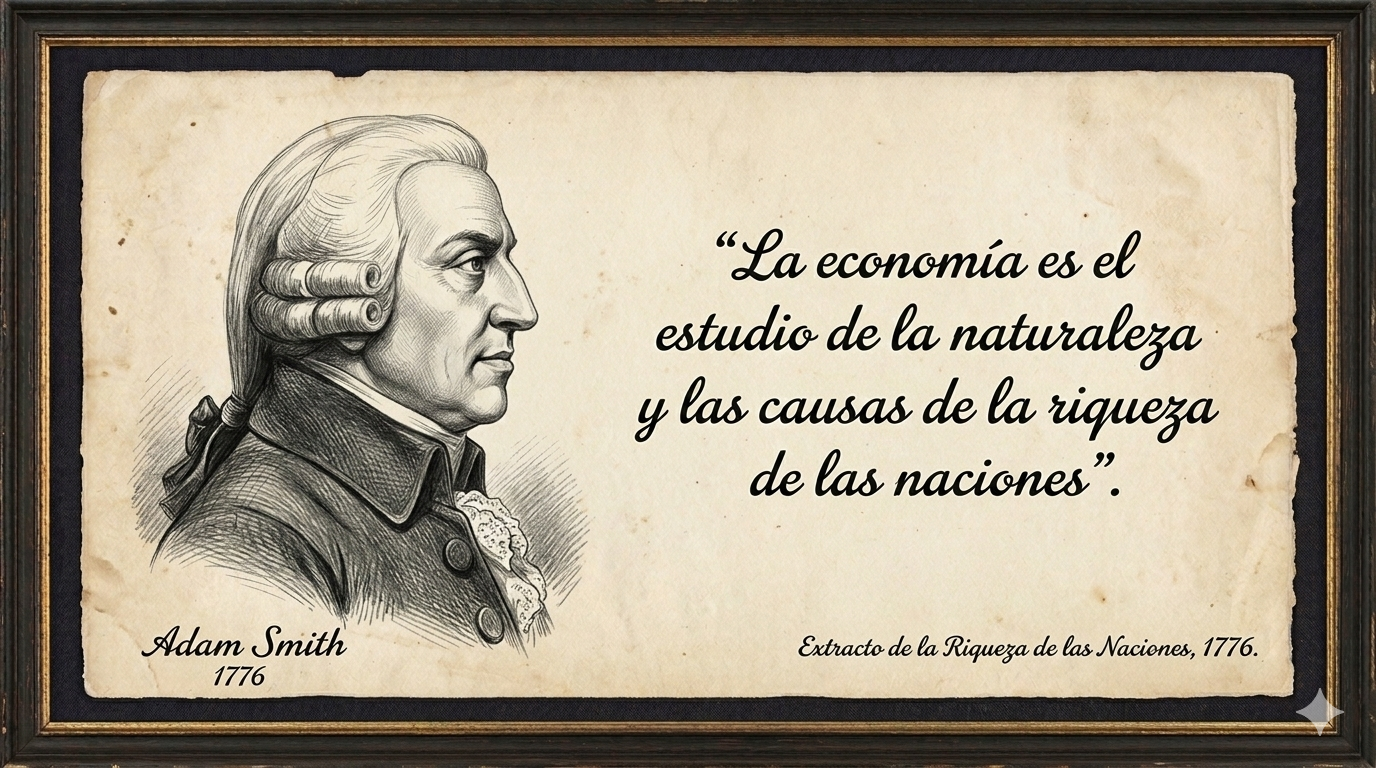
\includegraphics[keepaspectratio]{assets/adam-smith.png}}\end{minipage}%
%
\begin{minipage}{0.50\linewidth}
\pandocbounded{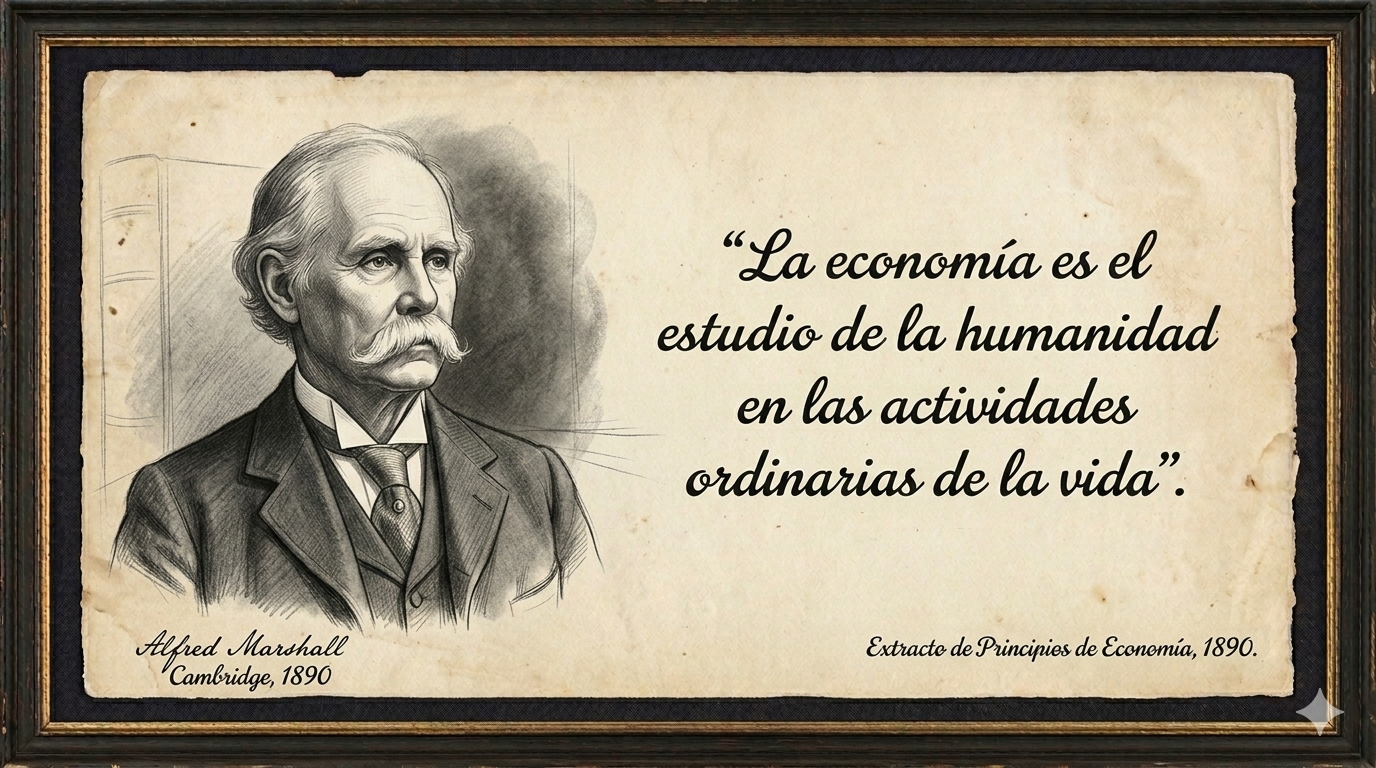
\includegraphics[keepaspectratio]{assets/alfred-marshal.png}}\end{minipage}%
\newline
\begin{minipage}{0.50\linewidth}
\pandocbounded{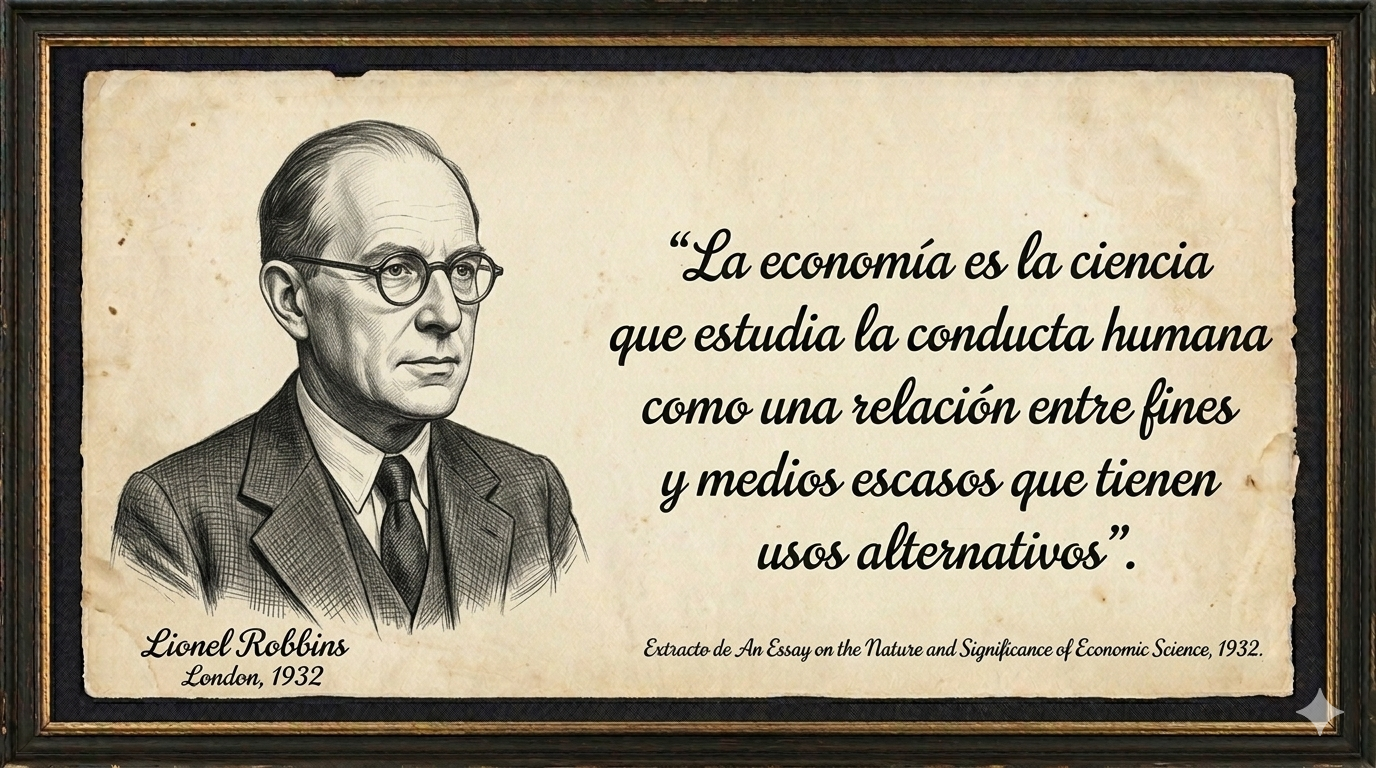
\includegraphics[keepaspectratio]{assets/lionel-robbins.png}}\end{minipage}%
%
\begin{minipage}{0.50\linewidth}
\pandocbounded{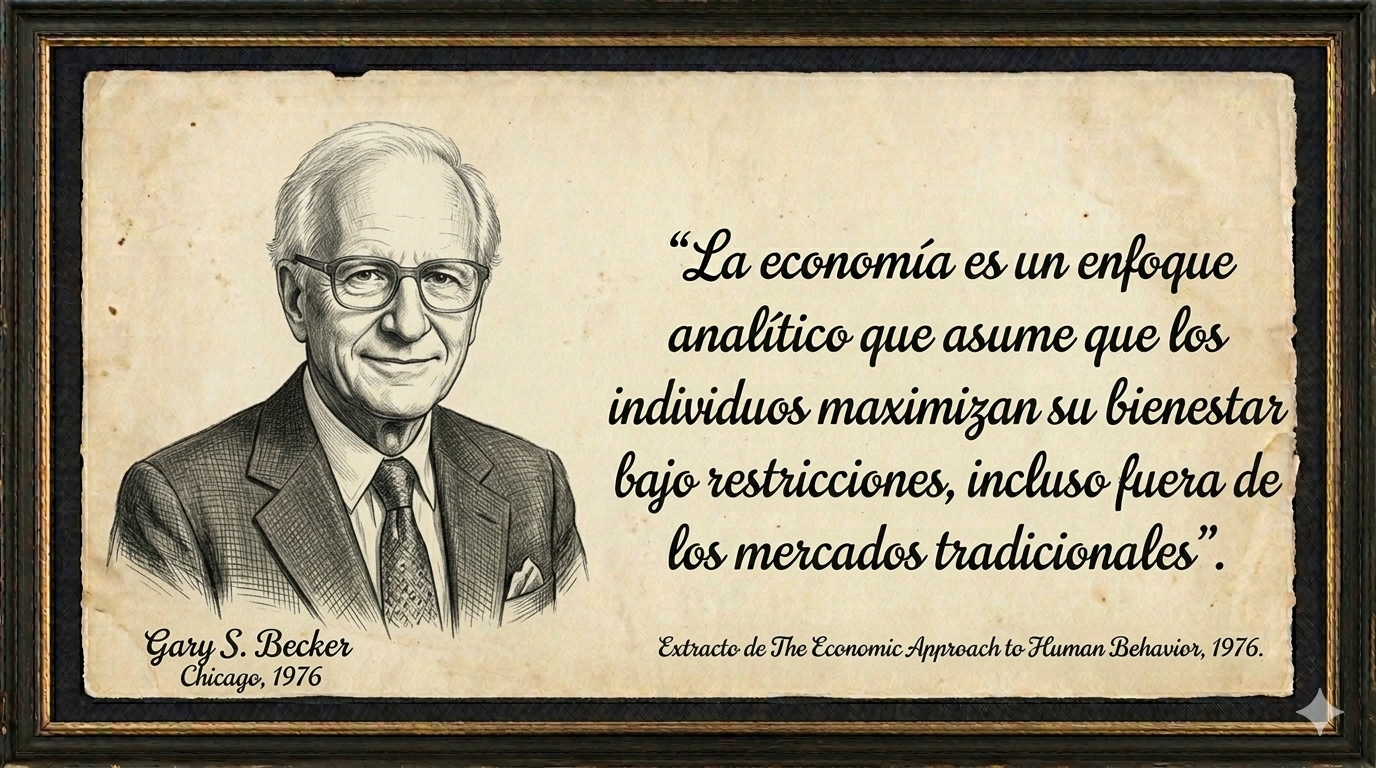
\includegraphics[keepaspectratio]{assets/gary-becker.png}}\end{minipage}%
\newline
\begin{minipage}{0.50\linewidth}
\pandocbounded{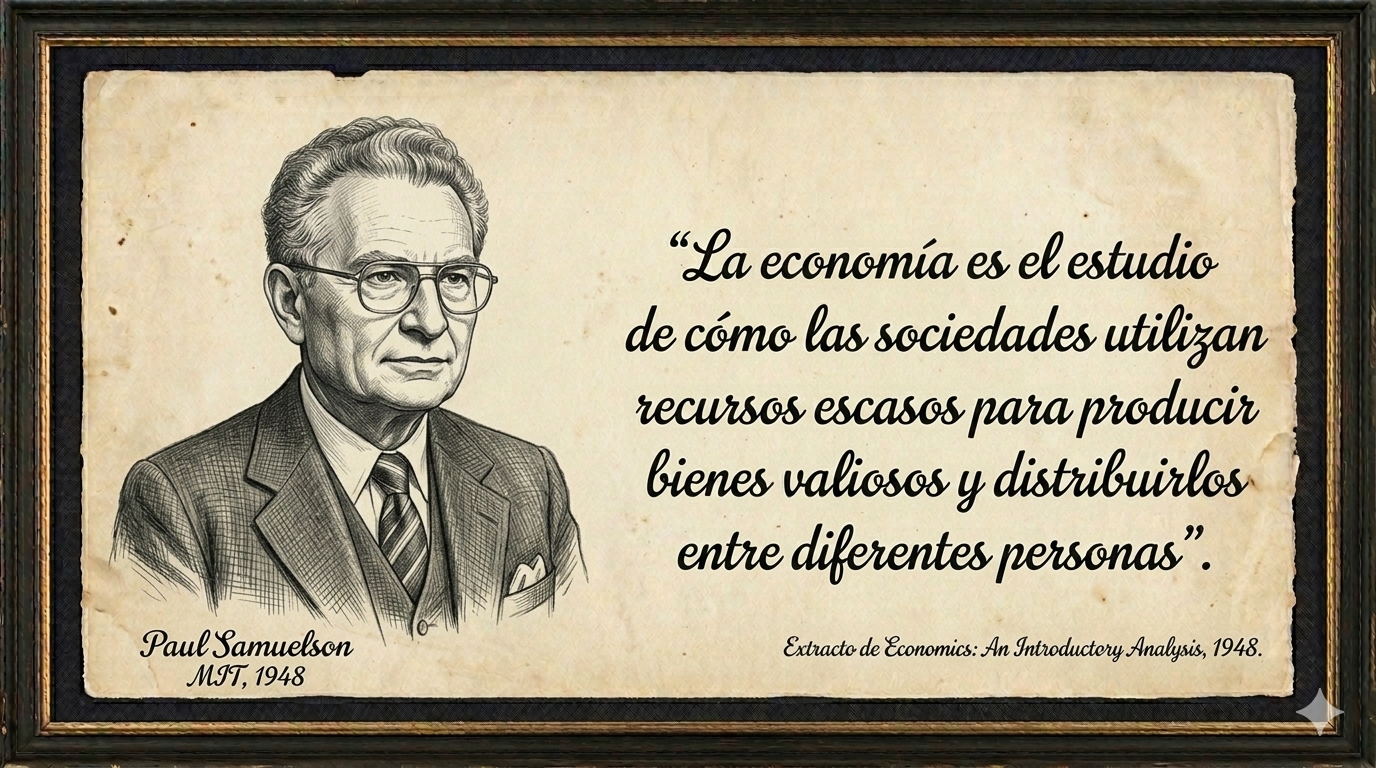
\includegraphics[keepaspectratio]{assets/paul-samuelson.png}}\end{minipage}%
%
\begin{minipage}{0.50\linewidth}
\pandocbounded{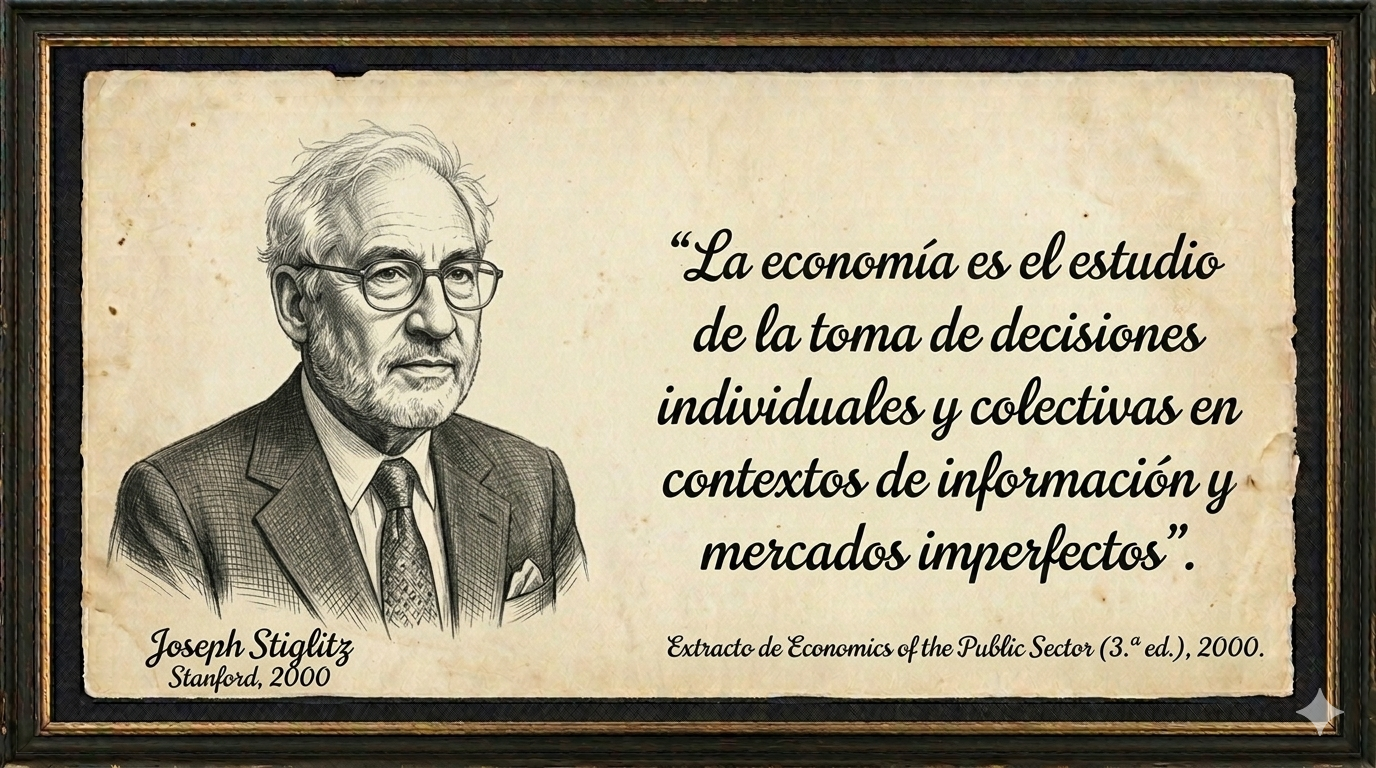
\includegraphics[keepaspectratio]{assets/joseph-stiglitz.png}}\end{minipage}%

\end{figure*}%

\begin{tcolorbox}[enhanced jigsaw, breakable, toprule=.15mm, colframe=quarto-callout-note-color-frame, leftrule=.75mm, opacityback=0, colback=white, bottomrule=.15mm, left=2mm, arc=.35mm, rightrule=.15mm]
\begin{minipage}[t]{5.5mm}
\textcolor{quarto-callout-note-color}{\faInfo}
\end{minipage}%
\begin{minipage}[t]{\textwidth - 5.5mm}

\vspace{-3mm}\textbf{¿Es la economía una ciencia?}\vspace{3mm}

La economía se considera una ciencia, pero es una ciencia social, no una
ciencia exacta como la física, la matemática o la química. La economía
combina métodos científicos (datos, modelos, hipótesis) con el arte
(juicio, política) debido a la complejidad del comportamiento humano,
por lo que se centra más en mejorar la comprensión que en la predicción
exacta. Los propios economistas tienen opiniones diversas, algunos
enfatizan su rigor científico a través de pruebas empíricas y otros
señalan sus limitaciones, distinguiéndola de las ciencias naturales,
donde los experimentos controlados son más fáciles. Por ejemplo, los
avances en el big data, la tecnología y la inteligencia artificial
permiten un análisis más sofisticado de sistemas complejos.

Sin embargo, a algunos críticos les preocupa que calificarla de ciencia
dura fomente el exceso de confianza y el dogmatismo, careciendo de una
verdadera apertura científica a métodos diversos. De hecho, varias
personalidades y grupos han pedido la abolición del Premio Nobel de
Economía, entre ellos el premio Nobel Gunnar Myrdal, el exministro de
Finanzas sueco Kjell-Olof Feldt y académicos como Bo Rothstein, que
argumentan que otorga una autoridad indebida a las ``ciencias blandas'',
promueve ideologías específicas (a menudo de derecha), y crea un ``aura
de certeza'' en un campo cargado de valores, lo que entra en conflicto
con la verdadera intención de Nobel.

\href{https://developingeconomics.org/2024/10/22/the-nobel-illusion-why-the-nobel-prize-in-economics-needs-to-be-abolished/}{\emph{Sherpa,
D., (2024). ``The Nobel Illusion: Why the Nobel Prize in Economics Needs
to be Abolished. October 22. Developing Economics}}

\href{https://www.pbs.org/newshour/economy/samuelson-on-whether-economics}{\emph{PBS
News (2009). Samuelson on Whether Economics Is a Science. December 24.}}

\end{minipage}%
\end{tcolorbox}

\begin{tcolorbox}[enhanced jigsaw, breakable, toprule=.15mm, colframe=quarto-callout-note-color-frame, leftrule=.75mm, opacityback=0, colback=white, bottomrule=.15mm, left=2mm, arc=.35mm, rightrule=.15mm]
\begin{minipage}[t]{5.5mm}
\textcolor{quarto-callout-note-color}{\faInfo}
\end{minipage}%
\begin{minipage}[t]{\textwidth - 5.5mm}

\vspace{-3mm}\textbf{¿Qué hacen los economistas?}\vspace{3mm}

Como dijo una vez el educador canadiense Laurence Peter: \emph{``Un
economista es un experto que mañana sabrá por qué las cosas que predijo
ayer no sucedieron hoy''}.

Hablando más en serio, los economistas desempeñan múltiples funciones en
la sociedad, y en la República Dominicana su trabajo es clave para el
diseño de políticas públicas, el funcionamiento del sector privado y la
comprensión de los problemas sociales y económicos del país.

En el sector público, los economistas cumplen un rol central como
asesores de política económica. Trabajan en instituciones como el Banco
Central, el Ministerio de Hacienda, la Superintendencia de Banco, el
Banco de Reservas, la Dirección General de Impuestos Internos (DGII) y
la Dirección General de Aduanas (DGA) donde participan en la formulación
de políticas fiscales, monetarias, tributarias y de desarrollo. Sus
análisis ayudan a decidir cómo asignar los recursos públicos, cómo
responder a choques externos y cómo promover la estabilidad
macroeconómica en una economía pequeña y abierta como la dominicana.

En el sector privado, los economistas apoyan la toma de decisiones
empresariales mediante estudios de mercado, análisis de costos,
proyecciones de demanda y evaluación de inversiones. También participan
en el sistema financiero, evaluando riesgos, diseñando productos y
analizando el comportamiento de los mercados.

Algunos economistas trabajan en el extranjero para empresas con
importantes operaciones internacionales y para organizaciones
internacionales como el Banco Mundial, el Fondo Monetario Internacional
y las Naciones Unidas. Además, muchos economistas dominicanos se
desempeñan como investigadores y académicos, generando conocimiento
sobre temas como informalidad laboral, desigualdad regional,
productividad o desarrollo sostenible. Finalmente, otros cumplen un rol
educativo y comunicador, explicando fenómenos económicos al público,
contribuyendo al debate nacional y fortaleciendo la cultura económica
del país.

\end{minipage}%
\end{tcolorbox}

\section{Principios del análisis
económico}\label{principios-del-anuxe1lisis-econuxf3mico}

\subsection{Las personas enfrentan
disyuntivas}\label{las-personas-enfrentan-disyuntivas}

Las disyuntivas (trade-offs) son conceptos fundamentales en economía por
su rol en el estudio de cómo los individuos, las empresas y las
sociedades toman decisiones para satisfacer necesidades con recursos
limitados. Una disyuntiva se refiere a una situación en la que es
necesario decidir renunciar o sacrificar una cosa para conseguir otra.
Cuando no se puede tener todo a la vez, se enfrenta una disyuntiva.

Por ejemplo, pensemos en elegir qué comer: cocinar en casa suele suponer
un ahorro, pero requiere más tiempo. Por el contrario, pedir comida para
llevar ahorra tiempo, pero cuesta más dinero. Tomar este tipo de
decisiones implica sopesar los beneficios y los costos de las distintas
opciones, lo que inevitablemente requiere afrontar disyuntivas y, en
última instancia, identificar la mejor alternativa.

El economista y comentarista político estadounidense Thomas Sowell
(2002, 2013) dijo: ``No hay soluciones a los problemas económicos, solo
hay disyuntivas''.

Las disyuntivas en economía están en todas partes, incluidas las
elecciones que hacen los consumidores al comprar bienes y servicios, las
decisiones que toman las empresas al invertir en nuevas oportunidades o
elaborar planes estratégicos. Los gobiernos también enfrentan
disyuntivas. Por ejemplo, cuando el gobierno dominicano decidió designar
el 4\% del PIB a la educación, tiene que sacrificar la inversión en
otras áreas que podría haber hecho con ese dinero, como gastarlo en la
defensa nacional, construir carreteras o pagar la deuda pública.

\subsection{Toda decisión tiene un costo de
oportunidad}\label{toda-decisiuxf3n-tiene-un-costo-de-oportunidad}

El costo de oportunidad es uno de los conceptos más importantes de la
economía. Se define como el valor de la mejor alternativa a la que se
renuncia cuando se toma una decisión. En otras palabras, cada vez que
elegimos algo, estamos dejando de lado otra opción. Por consiguiente, el
verdadero costo no es solo el dinero que gastamos, sino lo que
sacrificamos para tomar la decisión.

Este concepto es clave porque los recursos ---como el tiempo, el dinero
y el trabajo--- son limitados. Por eso, personas, empresas y gobiernos
deben pensar no solo en lo que obtienen con una decisión, sino también
en lo que dejan de ganar.

Por ejemplo, imaginemos que en la República Dominicana un joven con
educación secundaria puede ganar en promedio alrededor de RD\$15,000
mensuales, mientras que uno con educación universitaria puede ganar
cerca de RD\$35,000 mensuales. Si el joven decide trabajar
inmediatamente después del bachillerato y no ir a la universidad, su
costo de oportunidad es el mayor salario futuro que podría haber
obtenido con estudios universitarios, es decir RD\$ 35,000 mensuales.
Aunque gana hoy estaría ganando RD\$15,000 mensuales, con dejar la
universidad estaría renunciando a mejores ingresos en el futuro.

Para ilustrar el impacto del concepto de costo de oportunidad,
utilizaremos un instrumento grafico llamado la frontera de posibilidades
de producción (FPP). La FPP muestra las combinaciones máximas de dos
bienes que una economía puede producir cuando utiliza plenamente sus
recursos y tecnología. La relación con el costo de oportunidad es
directa: cada punto de la FPP refleja cuánto de un bien debe
sacrificarse para obtener más del otro.

Cuando una economía se mueve a lo largo de la FPP, aumentar la
producción de un bien implica renunciar a parte de la producción del
otro. Esa cantidad sacrificada es precisamente el costo de oportunidad.
Por ejemplo, si para producir más alimentos se reduce la producción de
ropa, la ropa dejada de producir representa el costo de oportunidad de
producir más alimentos.

Además, la forma típica cóncava de la FPP ilustra el costo de
oportunidad creciente: a medida que se produce más de un bien, se deben
sacrificar cantidades cada vez mayores del otro, porque los recursos no
son igualmente eficientes en todas las actividades. Así, la FPP permite
visualizar de manera clara y concreta el concepto de costo de
oportunidad en una economía.

La FPP representa la necesidad de elegir entre los 2 bienes. Producir
más de un bien supone producir menos de otro. La razón es que como todos
los factores están siendo utilizados, si queremos producir más peces
tendremos que usar parte de los trabajadores y otros recursos que
usábamos para recolectar vegetales, y por tanto obtendremos menos
cantidad. El coste de oportunidad de producir más de un bien es
renunciar a producir el otro.

Así, pasar de la combinación A a la combinación C nos permite producir
20kg de peces más, pero tendremos que renunciar a 15kg de vegetales. El
coste de oportunidad de 20kg de peces es renunciar a 15kg de vegetales
en ese punto de la frontera. De la misma manera, pasar de la combinación
E a la combinación D nos permite producir 30kg de vegetales más, pero
tenemos que renunciar a 10kg de peces. \ul{El coste de oportunidad de
30kg de peces es renunciar a 10 de vegetales en ese punto de la
frontera}.

\begin{figure}[H]

{\centering \pandocbounded{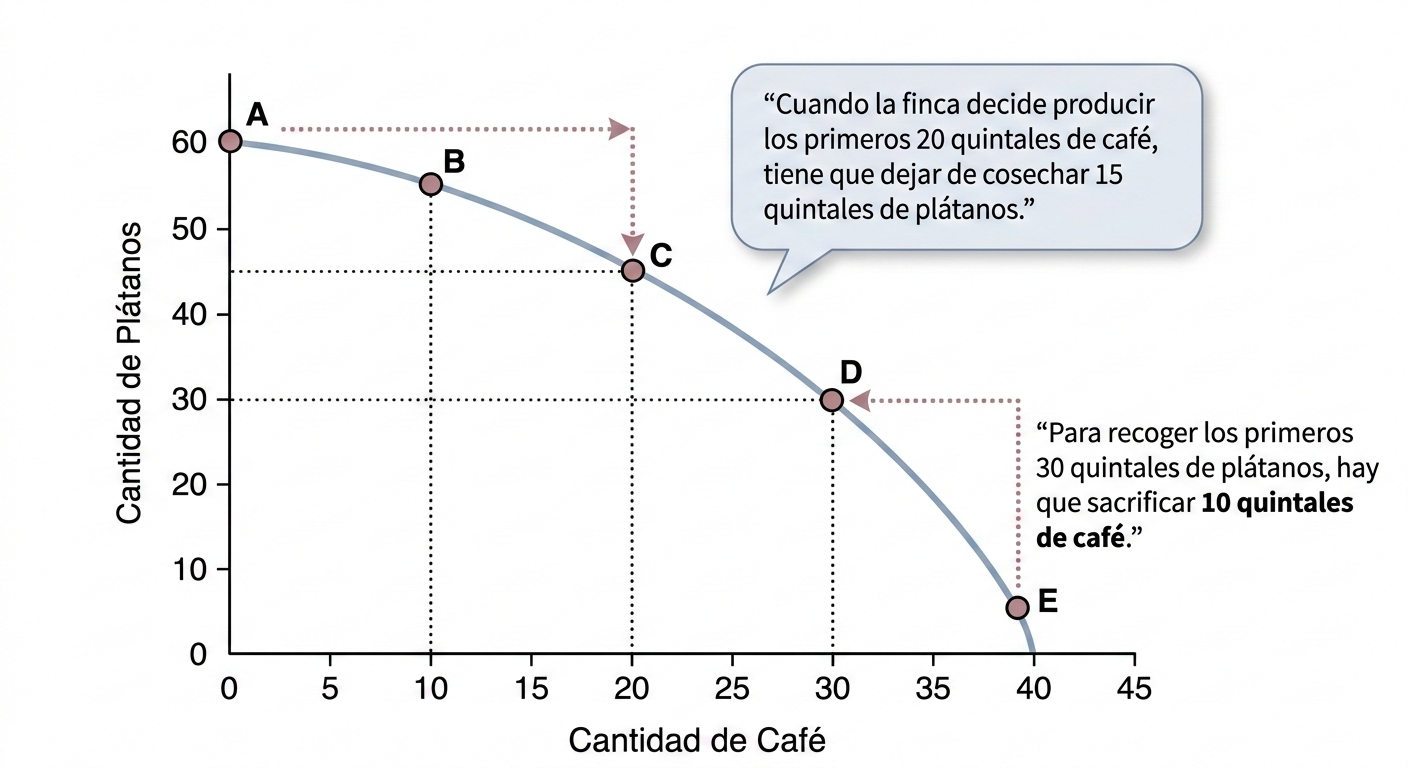
\includegraphics[keepaspectratio]{assets/cap1-fpp-platano-cafe.png}}

}

\caption{Frontera de posibilidades de producción}

\end{figure}%

La frontera de posibilidades también nos permite entender el concepto de
eficiencia que hemos visto en este tema. A un país le ocurre lo mismo lo
que a mi alumna María, tiene una serie de recursos como trabajadores,
máquinas y recursos naturales, y puede emplearlos de manera más o menos
eficiente.

La FPP nos muestra LAS COMBINACIONES EFICIENTES de la aldea. Es decir,
todos los puntos de la curva de FPP son eficientes (utilizamos todos los
recursos disponibles de la mejor forma posible), con nuestra tecnología
y nuestros factores productivos, estamos produciendo lo máximo posible.

Cuando los habitantes de la aldea pescan 20 kg de peces y recolectan
45kg de vegetales están siendo eficientes porque no pueden conseguir una
combinación igual o mejor en ambos bienes (no se puede pescar 30 kg y
recolectar 50kg por ejemplo).

De esta manera la FPP nos permite separar dos regiones.

\begin{itemize}
\item
  \ul{Puntos ineficientes.} Aquellos puntos que se encuentran por debajo
  de la curva, representan combinaciones ineficientes pues se están
  despilfarrando recursos (como cuando María memorizaba y perdía dos
  horas de estudio). Es decir, o bien no estamos usando recursos o bien
  los usamos de manera incorrecta (como María cuando elegía una mala
  técnica de estudio). Si en nuestra aldea se pescaran 20 peces y se
  recolectaran 20 vegetales (combinación F) se estaría siendo
  ineficiente, ya que si usamos todos los recursos que tenemos podríamos
  pescar 20 peces y recolectar 45 vegetales (combinación C). La
  combinación 20 peces y 20 vegetales es por tanto ineficiente y se
  representa en el punto F por debajo de la curva.
\item
  \ul{Puntos inalcanzables.} Aquellos puntos que se encuentra por encima
  de la curva son posiciones inalcanzables con los factores productivos
  y la tecnología disponible en ese momento dado. En nuestra aldea no
  podemos pescar 30 peces y recolectar 40 vegetales (punto G). Esa
  combinación es inalcanzable con los recursos y tecnología que tenemos.
  Sin embargo, con el paso del tiempo, las posiciones inalcanzables se
  pueden llegar a alcanzar si suceden una serie de circunstancias. Es lo
  que llamamos crecimiento económico.
\end{itemize}

\pandocbounded{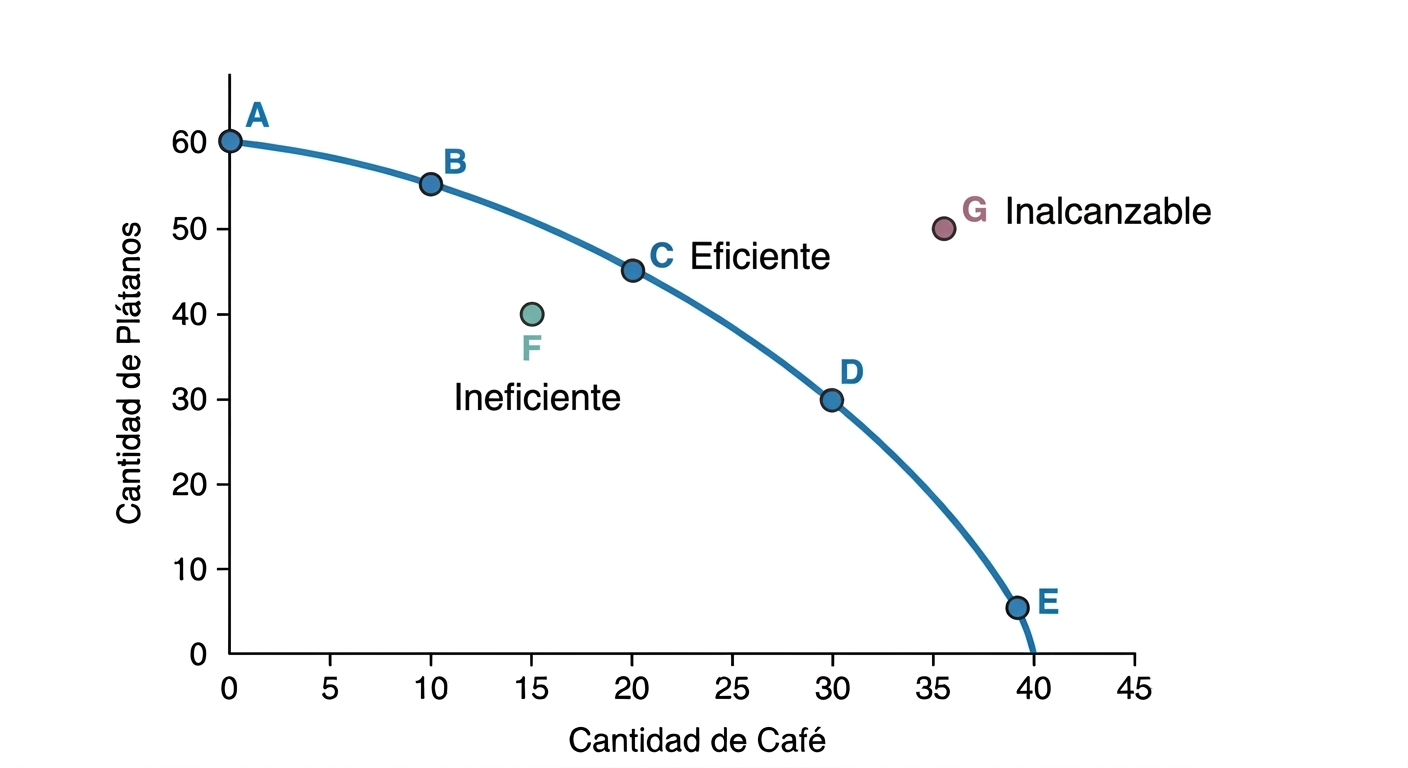
\includegraphics[keepaspectratio]{assets/cap1-fpp-categorias.png}}

\subsection{La persona racional piensa en términos
marginales}\label{la-persona-racional-piensa-en-tuxe9rminos-marginales}

La racionalidad en economía es la idea de que los agentes (individuos,
empresas, gobierno) toman decisiones lógicas para maximizar su bienestar
(utilidad, beneficios) evaluando costos y beneficios, eligiendo la mejor
opción disponible. Sin embargo, el desarrollo reciente de la economía
conductual liderada por el profesor Richard Thaler, premio nobel en
economía 2017, ha demostrado que las decisiones reales son limitadas por
información imperfecta y los sesgos psicológicos, limitando el ejercicio
de la racionalidad a buscar una solución lo ``suficientemente buena'',
en lugar de la perfecta. Sobre esto profundizaremos más adelante.

En economía, pensar en términos marginales significa tomar decisiones
comparando los beneficios y costos adicionales de tomar una determinada
decisión en lugar de evaluar los beneficios y costos totales. Este
enfoque reconoce que la mayoría de las decisiones económicas no son de
``todo o nada'', sino incrementales: producir una unidad más, trabajar
una hora adicional o gastar un peso extra. Un principio central de la
economía establece que una acción debe realizarse si su beneficio
marginal es mayor o igual a su costo marginal.

Pensar en el margen es fundamental para entender el comportamiento
racional de individuos, empresas y gobiernos. Por ejemplo, una persona
no decide si trabajar o no únicamente en función de su salario total
mensual, sino considerando si el ingreso adicional por una hora extra de
trabajocompensa el cansancio, el tiempo libre perdido o el costo del
transporte. Este razonamiento marginal permite explicar por qué las
decisiones cambian cuando cambian los incentivos, aun cuando los niveles
totales permanezcan constantes.

En la República Dominicana, un primer ejemplo se observa en las empresas
turísticas, como hoteles y restaurantes. Un hotel decide si aceptar una
reserva adicional evaluando si el ingreso marginal de ocupar una
habitación más supera el costo marginal de limpieza, energía y personal.
Incluso si el hotel ya cubrió sus costos fijos, la decisión de vender
una habitación extra a un precio reducido puede ser rentable si el
beneficio marginal es positivo.

\begin{tcolorbox}[enhanced jigsaw, breakable, toprule=.15mm, colframe=quarto-callout-note-color-frame, leftrule=.75mm, opacityback=0, colback=white, bottomrule=.15mm, left=2mm, arc=.35mm, rightrule=.15mm]
\begin{minipage}[t]{5.5mm}
\textcolor{quarto-callout-note-color}{\faInfo}
\end{minipage}%
\begin{minipage}[t]{\textwidth - 5.5mm}

\vspace{-3mm}\textbf{La falacia del costo hundido}\vspace{3mm}

En economía, un costo hundido es un costo que ya se ha incurrido y que
no puede recuperarse, independientemente de las decisiones que se tomen
en el futuro. Debido a esta característica, los costos hundidos no
deberían influir en las decisiones económicas racionales, ya que solo
los costos y beneficios futuros son relevantes para elegir entre
alternativas. Sin embargo, en la práctica, personas y organizaciones
suelen cometer el error de considerar estos costos pasados, lo que
conduce a decisiones ineficientes.

La falacia del costo hundido es un error común que se comente cuando se
sigue invirtiendo en un proyecto o decisión que no es rentable,
simplemente porque ya se ha gastado mucho tiempo, dinero o esfuerzo en
él, en lugar de evaluar si continuar es la mejor opción. Es la tendencia
a no querer ``perder'' lo invertido, incluso si la lógica indica que es
mejor abandonar y minimizar pérdidas.

Un ejemplo de esta situación es el caso del Hotel ``El Prado'' en el
Malecón de Santo Domingo, paralizado en los años noventa por un problema
de caverna subterránea que requirió costosas inyecciones de hormigón,
llevando a la quiebra del banco promotor. El proyecto, ubicado a pocos
metros de la esquina de las avenidas 30 de mayo y Máximo Gómez, buscaba
construir un hotel de 5 estrellas con 20 niveles y restaurante
giratorio.

\begin{figure}[H]

{\centering \pandocbounded{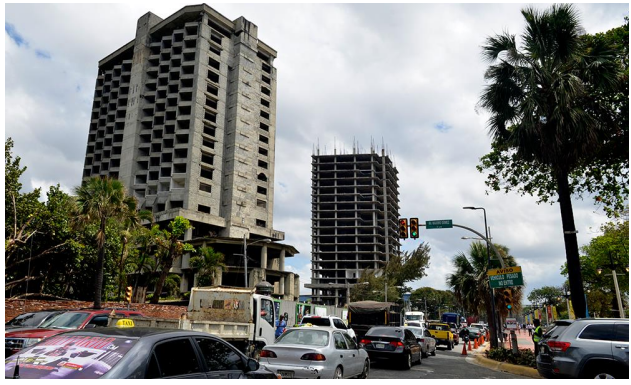
\includegraphics[keepaspectratio]{assets/cap1-edificios-gomez.png}}

}

\caption{Puntos}

\end{figure}%

El alto costo de esta reparación necesaria para terminar el proyecto fue
el factor clave para su abandono definitivo. Este caso ilustra
perfectamente como un problema técnico (la caverna) se transformó en un
desastre financiero y legal, dejando un gran costo hundido. En este
caso, la decisión de abandonar el proyecto se tomó demasiado tarde,
dejando hoy una enorme estructura abandonada en medio del malecón de
Santo Domingo.

\end{minipage}%
\end{tcolorbox}

\subsection{Las personas responden a
incentivos}\label{las-personas-responden-a-incentivos}

Un incentivo es cualquier factor que motiva o desalienta una determinada
decisión o comportamiento, ya sea de naturaleza económica, social o
moral. Debido a que los individuos buscan mejorar su bienestar dadas sus
restricciones, tienden a ajustar su comportamiento cuando cambian los
costos y beneficios asociados a sus decisiones.

En economía, los incentivos suelen ser monetarios (como salarios,
precios, impuestos o subsidios), pero también pueden ser no monetarios,
como el prestigio, la seguridad, el tiempo libre o el cumplimiento de
normas sociales. Este principio parte de la idea de que, al tomar
decisiones, las personas comparan costos y beneficios y ajustan su
comportamiento cuando estos cambian.

Las personas responden a incentivos comparando beneficios y costos
marginales. Cuando el beneficio esperado de una acción aumenta o su
costo disminuye, es más probable que esa acción se realice. Por el
contrario, si una política encarece una conducta o reduce sus
beneficios, las personas tienden a evitarla. Por ello, los economistas
prestan especial atención a cómo las políticas públicas, las reglas del
mercado o las condiciones económicas alteran los incentivos y, en
consecuencia, los resultados económicos. Ignorar los incentivos puede
llevar a políticas ineficientes o con efectos no deseados.

En la República Dominicana, si el gobierno reduce costos de registro y
ofrece incentivos fiscales a las pequeñas y medianas empresas, más
negocios podrían encontrar más atractivo operar en la formalidad. En
cambio, altos impuestos o trámites complejos generan incentivos para
permanecer en la informalidad. Algo similar sucede cuando el gobierno
subsidia los precios de la gasolina o el gas licuado de petróleo (GLP),
los consumidores tienden a usar más sus vehículos o a consumir más
energía, porque el costo por unidad es menor. En cambio, cuando los
precios suben, las personas buscan alternativas, como reducir viajes o
usar transporte público. Estos casos muestran claramente cómo los
incentivos influyen en las decisiones cotidianas.

\section{Las áreas de estudio de la
economía}\label{las-uxe1reas-de-estudio-de-la-economuxeda}

El estudio de la economía se divide tradicionalmente en dos grandes
áreas: la microeconomía y la macroeconomía. Aunque analizan la realidad
económica desde distintos niveles, ambas son complementarias y
necesarias para comprender cómo funciona una economía en su conjunto.

\subsection{Microeconomía}\label{microeconomuxeda}

La microeconomía se centra en el comportamiento de los agentes
individuales (hogares, empresas y sectores de la economía) y en cómo
toman decisiones. Por ejemplo, la microeconomía se aplica al estudio del
comportamiento de los consumidores, como la forma en que los hogares
dominicanos ajustan su consumo de alimentos, transporte o electricidad
cuando cambian los precios o sus salarios. Este análisis permite
comprender cómo se forman los precios y cómo reaccionan los agentes
económicos ante distintos incentivos.

A nivel empresarial, la microeconomía nos ayuda a entender el impacto
que tiene un cambio en el costo de las materias primas sobre el precio
de venta al consumidor de cualquier bien o servicio. La microeconomía
también nos ayuda a entender cómo el sector turístico se ajusta al
impacto que tiene un aumento del precio de los pasajes aéreos sobre la
llegada de visitantes al país o la proliferación del sargazo en las
playas sobre los costos de operación de los hoteles.

\subsection{Macroeconomía}\label{macroeconomuxeda}

La macroeconomía, en cambio, estudia el comportamiento de la economía en
su conjunto y se centra en el análisis de variables agregadas, como el
producto interior bruto (PIB), la inflación, el desempleo y las
políticas económicas que el gobierno implementa para influir en estos
indicadores. A diferencia de la microeconomía, la macroeconomía se
centra en el análisis de la economía desde una perspectiva global,
examinando cómo interactúan todos los mercados en su conjunto y las
relaciones entre países en lo que respecta al comercio y la inversión
internacional. Este enfoque permite identificar patrones, ciclos
económicos y tendencias que afectan a millones de personas y a la
estabilidad de los sistemas económicos.

Los gobiernos utilizan el análisis macroeconómico para formular
políticas fiscales (impuestos y gasto público) y monetarias (control de
la oferta de dinero y las tasas de interés). Estas políticas tienen como
objetivo estabilizar la economía, fomentar el crecimiento y reducir el
desempleo. Las empresas también utilizan el análisis macroeconómico para
planificar inversiones, fijar precios y determinar estrategias de
mercado en función del entorno económico. Una economía estable es
fundamental para el bienestar de la población. En concreto, la
macroeconomía ayuda a identificar y mitigar los riesgos de crisis
económicas, como las recesiones o la hiperinflación.

\section{Los enfoques de la
economía}\label{los-enfoques-de-la-economuxeda}

En economía, suelen distinguirse dos grandes enfoques para su estudio:
el enfoque positivo y el enfoque normativo. Ambos son complementarios y
permiten analizar la realidad económica desde perspectivas distintas,
pero relacionadas.

El enfoque positivo se centra en describir y explicar cómo funciona la
economía en la práctica, para lo que utiliza datos, modelos y evidencia
empírica. Su objetivo es responder a preguntas del tipo «qué es» o «qué
ocurre si», evitando juicios de valor.

En la República Dominicana, el enfoque positivo se puede ilustrar con el
análisis del comportamiento de la inflación. Por ejemplo, un economista
puede estudiar cómo los cambios en los precios internacionales del
petróleo afectan a la inflación interna utilizando estadísticas del
Banco Central. Los resultados obtenidos nos indicarían numéricamente la
magnitud del cambio en la inflación cuando sube o baja el petróleo.

En contraste, el enfoque normativo se ocupa de evaluar los resultados
económicos y de proponer cómo debería funcionar la economía según
ciertos criterios de bienestar, equidad o justicia social, y responde a
preguntas como «¿qué debería ser?».

Este enfoque se aplica cuando se discuten políticas públicas y objetivos
sociales. Por ejemplo, si los sindicatos exigen a los empresarios un
aumento de salarios, un análisis con un enfoque normativo se centraría
en si el salario mínimo debería aumentarse para mejorar el nivel de vida
de los trabajadores, aunque ello pudiera implicar un posible aumento del
desempleo o de la inflación. En este caso, entran en juego juicios de
valor sobre equidad y bienestar.

En conjunto, el enfoque positivo aporta pruebas y comprensión, mientras
que el normativo orienta las decisiones de política económica. Ambos son
esenciales para analizar y afrontar los desafíos económicos de la
República Dominicana.

\section*{Preguntas de repaso}\label{preguntas-de-repaso}
\addcontentsline{toc}{section}{Preguntas de repaso}

\markright{Preguntas de repaso}

\begin{enumerate}
\def\labelenumi{\arabic{enumi}.}
\item
  ¿Por qué la escasez es el punto de partida del análisis económico?
\item
  ¿Cuál es la diferencia entre necesidades y deseos?
\item
  Explique con un ejemplo dominicano el concepto de disyuntiva.
\item
  ¿Qué es el costo de oportunidad y por qué es clave para tomar
  decisiones?
\item
  ¿Cómo la FPP ayuda a ilustrar el costo de oportunidad?
\item
  ¿Qué significa que una economía opere de manera eficiente?
\item
  ¿Por qué los costos hundidos no deberían influir en las decisiones
  racionales?
\item
  ¿Qué implica pensar en términos marginales?
\item
  ¿Cómo influyen los incentivos en el comportamiento de las personas y
  las empresas?
\item
  ¿En qué se diferencian la microeconomía y la macroeconomía, y por qué
  ambas son necesarias?
\end{enumerate}

\section*{Ejercicios}\label{ejercicios}
\addcontentsline{toc}{section}{Ejercicios}

\markright{Ejercicios}

\begin{enumerate}
\def\labelenumi{\arabic{enumi}.}
\item
  Identifique tres situaciones de escasez que sean importantes en el
  lugar donde vive (agua, mano de obra cualificada, electricidad,
  tierra, crédito). Explique cómo se refleja cada escasez en los precios
  o las colas, y proponga una política para reducirla. Utilice el coste
  de oportunidad para justificar su propuesta.
\item
  Una familia recibe RD\$ 12,000 en remesas este mes. Enumere tres usos
  alternativos y analice el costo de oportunidad de cada uno. ¿Qué
  opción tiene el mayor rendimiento esperado y por qué?
\item
  El salario mínimo en la República Dominicana varía según el tamaño de
  la empresa. ¿Cómo reconoce este diseño institucional las escaseces
  heterogéneas entre las empresas? ¿En qué condiciones podría esta
  diferenciación ralentizar la formalización?
\item
  Dibuje una PPF para «servicios turísticos» frente a «manufactura».
  ¿Qué inversiones públicas desplazarían la FPP hacia afuera para ambos
  bienes simultáneamente? Defienda su respuesta con ejemplos
  dominicanos.
\item
  Suponga que las llegadas de visitantes crecen un 5 \% el próximo año.
  Discuta los posibles cuellos de botella (agua, energía, transporte) y
  los costos de oportunidad de satisfacer ese aumento mediante (i) nueva
  capacidad frente a (ii) gestión de la demanda.
\item
  Describa algunas disyuntivas que enfrentan los siguientes actores:

  \begin{enumerate}
  \def\labelenumii{\arabic{enumii}.}
  \tightlist
  \item
    Una familia que está pensando en comprar un automóvil nuevo.
  \item
    Un miembro del Congreso que debe decidir cuánto gastar en parques
    acionales.
  \item
    El presidente de una empresa que debe decidir abrir o no una nueva
    1ábrica.
  \item
    El profesor que decide por cuánto tiempo preparar su clase.
  \item
    Alguien recién egresado de la universidad que decide si cursar o no
    una maestría.
  \end{enumerate}
\item
  Usted está tratando de decidir si debe tomar o no vacaciones. La mayor
  parte del costo de las vacaciones, como el avión, el hotel y dejar de
  recibir un salario, se mide en términos monetarios, pero los
  beneficios de las vacaciones son psicológicos. ¿Cómo podemos comparar
  los beneficios y los costos?
\item
  Usted está planeando pasar el sábado trabajando en un empleo de medio
  tiempo, pero un amigo lo invita a esquiar. ¿Cuál es el verdadero costo
  de ir a esquiar? Ahora suponga que usted había planeado pasar el día
  estudiando en la biblioteca. En este caso ¿cuál es el costo de ir a
  esquiar? Explique.
\item
  Usted gana \$100 apostando a un equipo de basquetbol. Ahora debe
  decidir entre gastar ese dinero o depositarlo en el banco por un año y
  ganar 5\% de interés. ¿Cuál es el costo de oportunidad de gastar los
  \$100 ahora?
\item
  La empresa que usted dirige invierte \$5 millones para desarrollar un
  nuevo producto, pero su desarrollo no está totalmente terminado. En
  una junta el personal de ventas le informó que el lanzamiento de
  productos parecidos de los competidores probablemente reducirá las
  ventas del nuevo producto a \$3 millones. Si cuesta un millón
  completar el desarrollo del producto y fabricarlo, ¿se debería seguir
  adelante con el proyecto? ¿Cuánto es lo más que se debe pagar para
  completarlo?
\end{enumerate}

\chapter{La economía como sistema}\label{la-economuxeda-como-sistema}

\chapter{Las teorías económicas y los
modelos}\label{las-teoruxedas-econuxf3micas-y-los-modelos}

\part{Microeconomía}

\chapter{Oferta y demanda}\label{oferta-y-demanda}




\end{document}
